\chapter{Proposed Smart Governance Framework}
This chapter synthesizes the computational findings into an actionable, evidence-based governance strategy for the Municipality of Bacolod. By bridging the gap between Deep Reinforcement Learning (DRL) outputs and socioeconomic realities, the evaluation uncovers the specific mechanisms that dictate solid waste management (SWM) success in the Philippine local government context \citep{Jimenez2025}. 

% Optional: Placeholder for a diagram showing the 4 pillars
\begin{figure}[h]
     \centering
     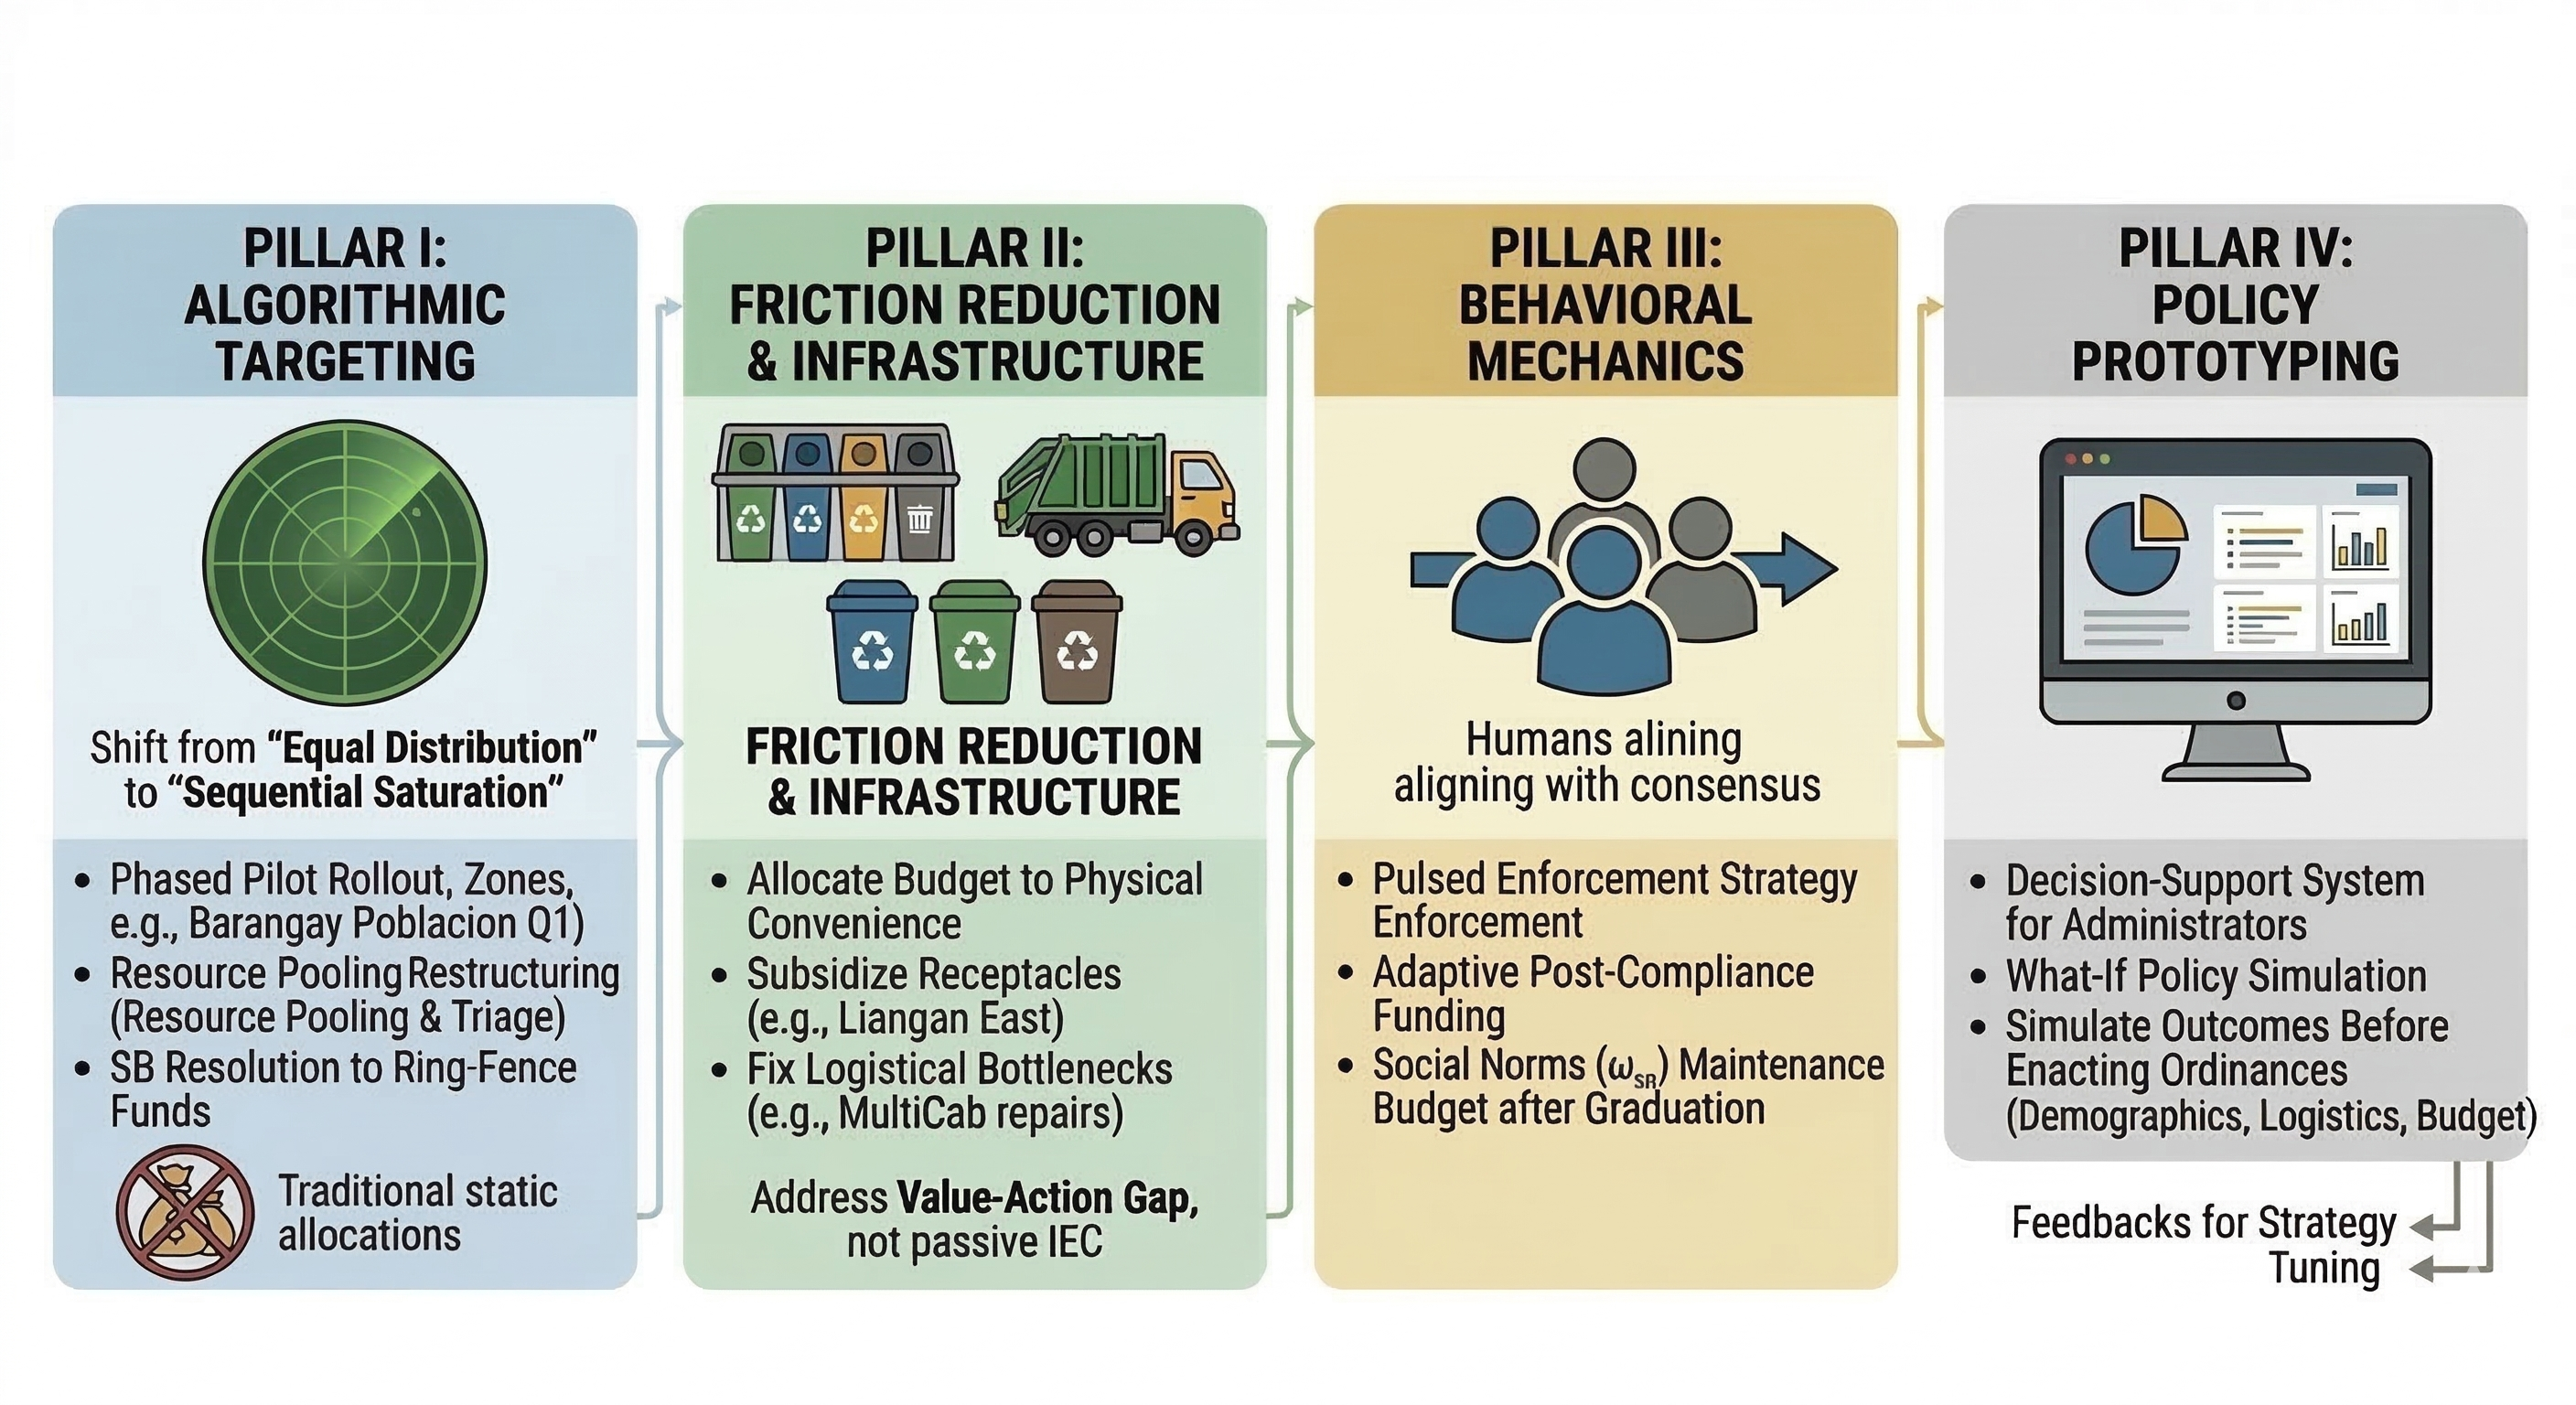
\includegraphics[width=0.8\textwidth]{images/proposed_framework.png}
     \caption{The Proposed Data-Driven Solid Waste Management (DD-SWM) Framework}
     \label{fig:framework}
 \end{figure}

Traditional environmental policy design in developing nations frequently suffers from the "implementation deficit"—a phenomenon where ambitious national mandates fail at the local level due to a mismatch between legislative intent and actual local capacity \citep{Howlett2019, Magno2021}. To transition from heuristic-based administration to predictive governance, this study proposes the \textbf{Data-Driven Solid Waste Management (DD-SWM) Framework}. This framework discards static, uniform budget allocations in favor of a dynamic, four-pillar model: Algorithmic Resource Targeting, Friction Reduction, Adaptive Behavioral Mechanics, and Predictive Prototyping.

\section{Pillar I: Algorithmic Resource Targeting}
The first pillar of the proposed framework addresses the critical structural flaw of ``Equal Distribution,'' frequently referred to in public administration as the ``peanut-buttering'' effect. Traditional administrative heuristics—wherein funds are spread evenly across all barangays—are often employed by local executives to maintain a veneer of political neutrality and avoid accusations of favoritism \citep{Cruz2020}. However, within the context of this simulation, such an approach is mathematically modeled as a mechanism of dilution \citep{Alphonso2024}. By distributing a limited budget equally across jurisdictions with vastly different needs, the Local Government Unit (LGU) ensures that the critical density of enforcement or incentives required to trigger behavioral change is never achieved in densely populated, highly resistant urban centers like Barangay Poblacion \citep{Villanueva2021}.

To resolve this dilution, the LGU must adopt a strategy of ``Sequential Saturation,'' which requires reframing the budget allocation process as a structured, phased rollout. The Mayor and the Municipal Environment and Natural Resources Office (MENRO) should justify concentrating the overwhelming majority of the municipal MOOE budget into the most resistant zones, such as Poblacion, during the initial phase. By treating high-density areas as ``Pilot Zones,'' the LGU can break the initial behavioral inertia and lock in social norms via the Social Norm Shield before rotating those resources to rural areas like Demologan \citep{Zheng2022b}. This approach aligns with the ``focal point'' theory of resource allocation, which posits that overwhelming a single node in a network creates positive spillover effects for adjacent jurisdictions \citep{Ostrom2010}.

Complementing this geographic concentration is the necessity for dynamic financial restructuring. The simulation data revealed severe fiscal disparities, with some jurisdictions operating on SWM budgets as low as \textpeso 15,000 annually. To achieve municipal-wide sustainability, the LGU must abandon static, historical appropriation ordinances in favor of a pooled resource model. By cross-subsidizing high-impact infrastructure in underfunded barangays based on quarterly algorithmic triage, the municipal government ensures that capital flows precisely where behavioral resistance is highest \citep{Abdallah2021, Krause2019}. Operationally, this transition requires the drafting of a Sangguniang Bayan (SB) Resolution to legally ring-fence funds for targeted saturation. In this administrative context, the computational model serves as a ``mathematical shield'' for the executive branch, depoliticizing the allocation process by providing a data-backed rationale for abandoning simultaneous equality in favor of systemic efficacy \citep{Nishimura2022}.

\section{Pillar II: Friction Reduction and Infrastructure}
The second pillar focuses on the physical environment and choice architecture, grounded in the results of the Global Sensitivity Analysis. The GSA confirmed that the ``Cost of Effort'' ($c_{\text{effort}}$) is the dominant inhibitor of compliance in Bacolod, accounting for approximately 79\% of total output variance \citep{Yazawa2025}. In contrast, the near-zero sensitivity of the ``Attitude'' parameter quantifies a distinct ``Value-Action Gap,'' wherein citizens may possess high environmental awareness yet fail to act due to systemic physical barriers \citep{Blake1999, Zhao2022}. These findings fundamentally indicate that passive Information, Education, and Communication (IEC) campaigns, such as flyers or radio broadcasts, will yield negligible returns if the underlying ``sludge'' or physical friction of segregation remains unaddressed \citep{Sunstein2019, Moeini2023}.

Consequently, the LGU must pivot its fiscal priorities from awareness generation to the enhancement of physical convenience. A primary intervention involves the direct subsidization of segregation receptacles in low-income zones. Interviews revealed that residents in economically vulnerable areas, such as Liangan East, often find even basic materials like sacks (\textit{sako}) prohibitively expensive. By relying on individual procurement, the LGU effectively penalizes the poor for non-compliance. Allocating funds to distribute free, standardized segregation bins to these households neutralizes the financial barrier to entry and simplifies the decision-making process for the agent \citep{Thaler2008}.

In addition to receptacle subsidies, the LGU must prioritize the resolution of logistical bottlenecks that force residents toward undesirable practices like illegal dumping or the use of unmanaged compost pits \citep{Premakumara2014}. This includes the urgent need for hardware maintenance, exemplified by the currently non-functional MultiCab in Barangay Liangan East. Ensuring that the physical act of waste disposal aligns seamlessly with the desired civic behavior is a prerequisite for any punitive measure. Within this framework, the LGU acknowledges that it cannot ethically or practically penalize a populace for failing to utilize infrastructure that is either non-functional or non-existent. By reducing $c_{\text{effort}}$ through direct physical support, the municipality allows the AI's optimized policy mix to take root in an environment designed for success.

\section{Pillar III: Adaptive Behavioral Mechanics}
The third pillar governs how the LGU applies pressure and rewards over time, moving away from rigid, permanent enforcement structures toward adaptive behavioral interventions.

\subsection{Calibrated Enforcement and Political Capital}
The simulation provides strong computational evidence that a "Pure Enforcement" strategy is politically brittle, triggering a "Political Collapse" by Quarter 2 due to extreme public backlash. Heavy-handed penalization without adequate infrastructure or prior behavioral conditioning traps the LGU in an unsustainable cycle of resentment, often resulting in electoral punishment for incumbent officials \citep{Weaver1986}. 

The proposed framework advises against uniform, draconian ticketing. Instead, MENRO should deploy citation tickets selectively during the initial "Saturation Phase" of a targeted barangay to shatter early resistance. Once compliance begins to rise, the LGU must immediately scale back punitive measures. This "pulsed enforcement" creates a psychological deterrent without exhausting municipal goodwill, allowing Political Capital to recover to a stable 1.0000 \citep{Ayres1992}.

\subsection{The Graduation Rule and the 70\% Tipping Point}
The HuDRL agent successfully discovered that civic behavior does not require perpetual, high-intensity municipal funding once it becomes culturally normalized. Complex contagion models suggest that once a critical mass adopts a behavior, the behavior becomes self-sustaining \citep{Centola2018}. The LGU must continuously monitor barangays until they cross this "Social Tipping Point," computationally identified in this study as approximately 70\% compliance.

Once a barangay breaches this threshold, peer pressure and internalized social norms ($\omega_{sn}$) naturally sustain the segregation behavior \citep{Andre2021}. The framework introduces the "Graduation Rule": upon reaching 70\% compliance, MENRO must drastically titrate that barangay's funding down to a fractional "Maintenance Budget." This budget is tuned solely to counter habit decay, freeing up massive fiscal capital to besiege the next resistant population center.

\section{Pillar IV: Predictive Policy Prototyping}
The final pillar cements the framework by providing the LGU with the computational tools required to sustain it. Traditionally, LGU appropriation ordinances are drafted based on static heuristics, historical precedent, and political intuition. This highlights the potential benefits of transitioning to a dynamic, "What-If" planning model, effectively introducing the concept of a "Digital Twin" for municipal public policy \citep{Batty2018}.

The "Bacolod Multi-View Simulation UI" developed in this study serves as a proof-of-concept for this pillar. While the current iteration is a research prototype, it demonstrates the profound utility of predictive modeling in public administration. By commissioning or internally developing localized decision-support systems based on this DRL architecture, future administrators will be able to input demographic shifts, vehicle logistics constraints, and shifting budget allocations to simulate policy outcomes \textit{before} enacting municipal ordinances \citep{Kitchin2014}. This minimizes the risk of unintended consequences, avoids the costly misallocation of public funds, and permanently shifts the LGU from a paradigm of reactive enforcement to one of proactive, evidence-based governance.